\documentclass[brazil]{beamer}
\usepackage{beamerthemesplit}
\usepackage[brazilian]{babel}
\usepackage[utf8]{inputenc}
\usepackage{color}
\usepackage{xcolor}
\usepackage{graphicx}
%\usepackage{subcaption}
\usepackage{float}
\usepackage{wrapfig}
\usepackage{amssymb}
\usepackage{amsmath}
\usepackage{fancybox}
\usepackage{ulem}
\usepackage{listings}
\usepackage{upquote}
\usetheme{JuanLesPins}
%\usetheme{Warsaw}
%\usetheme{CambridgeUS}
%\usetheme{Malmoe}


%\newcommand{\lyxline}[1][1pt]{%
%  \par\noindent%
%  \rule[.5ex]{\linewidth}{#1}\par}


\title{
  Projeto Ouroboros
}
\subtitle{
  Um sistema de integração automatizada entre C++ e
  linguagens de script
}
\author{Wilson Kazuo Mizutani e Fernando Omar Aluani}

\begin{document}

% ---------------------------------------------------------------------------- %
% Opções de listing usados para o código fonte
% Ref: http://en.wikibooks.org/wiki/LaTeX/Packages/Listings
\lstdefinelanguage{lua}
  {morekeywords={and,break,do,else,elseif,end,false,for,function,if,in,local,
     nil,not,or,repeat,return,then,true,until,while},
   morekeywords={[2]arg,assert,collectgarbage,dofile,error,_G,getfenv,
     getmetatable,ipairs,load,loadfile,loadstring,next,pairs,pcall,print,
     rawequal,rawget,rawset,select,setfenv,setmetatable,tonumber,tostring,
     type,unpack,_VERSION,xpcall},
   morekeywords={[2]coroutine.create,coroutine.resume,coroutine.running,
     coroutine.status,coroutine.wrap,coroutine.yield},
   morekeywords={[2]module,require,package.cpath,package.load,package.loaded,
     package.loaders,package.loadlib,package.path,package.preload,
     package.seeall},
   morekeywords={[2]string.byte,string.char,string.dump,string.find,
     string.format,string.gmatch,string.gsub,string.len,string.lower,
     string.match,string.rep,string.reverse,string.sub,string.upper},
   morekeywords={[2]table.concat,table.insert,table.maxn,table.remove,
   table.sort},
   morekeywords={[2]math.abs,math.acos,math.asin,math.atan,math.atan2,
     math.ceil,math.cos,math.cosh,math.deg,math.exp,math.floor,math.fmod,
     math.frexp,math.huge,math.ldexp,math.log,math.log10,math.max,math.min,
     math.modf,math.pi,math.pow,math.rad,math.random,math.randomseed,math.sin,
     math.sinh,math.sqrt,math.tan,math.tanh},
   morekeywords={[2]io.close,io.flush,io.input,io.lines,io.open,io.output,
     io.popen,io.read,io.tmpfile,io.type,io.write,file:close,file:flush,
     file:lines,file:read,file:seek,file:setvbuf,file:write},
   morekeywords={[2]os.clock,os.date,os.difftime,os.execute,os.exit,os.getenv,
     os.remove,os.rename,os.setlocale,os.time,os.tmpname},
   alsodigit = {.},
   sensitive=true,
   morecomment=[l]{--},
   morecomment=[s]{--[[}{]]},
   morestring=[b]",
   morestring=[d]',
   morestring=[s]{[[}{]]},
  }

\lstset{ %
  language=C++,                     % choose the language of the code
  basicstyle=\ttfamily\scriptsize,  % the size of the fonts that are used for the code
  numbers=left,                     % where to put the line-numbers
  numberstyle=\footnotesize,        % the size of the fonts that are used for the line-numbers
  stepnumber=1,                     % the step between two line-numbers. If it's 1 each line will be numbered
  numbersep=5pt,                    % how far the line-numbers are from the code
  showspaces=false,                 % show spaces adding particular underscores
  showstringspaces=false,           % underline spaces within strings
  showtabs=false,                   % show tabs within strings adding particular underscores
  %frame=single,                     % adds a frame around the code
  %framerule=0.6pt,
  tabsize=2,                        % sets default tabsize to 2 spaces
  captionpos=b,                     % sets the caption-position to bottom
  breaklines=true,                  % sets automatic line breaking
  breakatwhitespace=false,          % sets if automatic breaks should only happen at whitespace
  escapeinside={\%*}{*)},           % if you want to add a comment within your code
  %backgroundcolor=\color[rgb]{1.0,1.0,1.0}, % choose the background color.
  %rulecolor=\color[rgb]{0.8,0.8,0.8},
  keywordstyle=\color{blue}\bfseries,
  keywordstyle=[2]\color[rgb]{.4,0,.4}\bfseries,
  commentstyle=\color[rgb]{0,.6,0},
  stringstyle=\color{red},
  showstringspaces=false,
  upquote=true,
  extendedchars=true,
  %xleftmargin=10pt,
  %xrightmargin=10pt,
  %framexleftmargin=10pt,
  %framexrightmargin=10pt,
  morekeywords={[2]include,ifdef,define,ifndef,endif,nullptr}
}

\frame{
  \titlepage
  Orientador: Prof. Dr. Marco Dimas Gubitoso
}

\frame{\tableofcontents}

%-------------------------------------
\section{Introdução: Motivações e Objetivos}
%-------------------------------------
\frame{
  \begin{center}
  \LARGE 1. Introdução: Motivações e Objetivos
  \end{center}
}
%-------------------------------------
\begin{frame}[fragile]
  \frametitle{Sistema de \textit{scripts} da UGDK (2011)}
  \pause
  \begin{figure}
    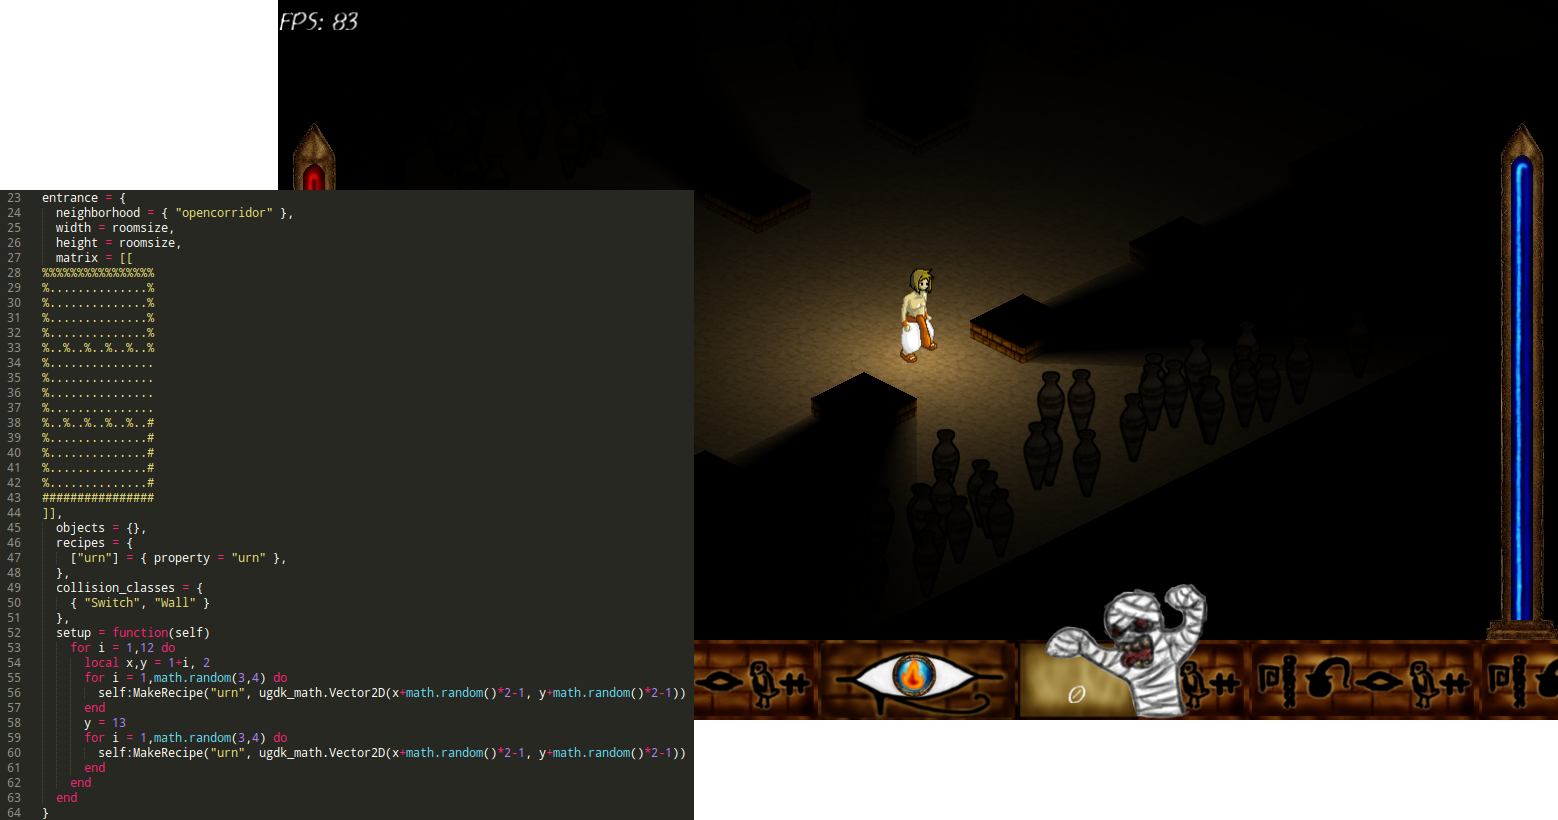
\includegraphics[width=.9\textwidth]{images/horus+sublime.png}
  \end{figure}
  \vspace{-10pt}
  \begin{itemize}
    \pause
    \item Interface única para diferentes linguagens de script
    \pause
    \item Exportação automatizada das classes em \texttt{C++} (via SWIG).
  \end{itemize}
\end{frame}
%-------------------------------------
\frame{
  \frametitle{Proposta de TCC (2013)}
  \pause
  \vspace{-20pt}
  \begin{center}
    Projeto Ouroboros
  \end{center}
  \vspace{20pt}
  \begin{itemize}
    \pause
    \item Resolver os problemas do SWIG
    \vspace{10pt}
    \pause
    \item Independência da UGDK
    \vspace{10pt}
    \pause
    \item Software Livre
  \end{itemize}
}
%%-------------------------------------
%\section{Alguns Conceitos}
%%-------------------------------------
%\frame{
%  \begin{center}
%  \LARGE 2. Alguns Conceitos
%  \end{center}
%}
%%-------------------------------------
%\begin{frame}[fragile]
%  \frametitle{Linguagens de programação}
%  \pause
%  Segundo Anthony A. Aaby:
%  \pause
%  \vspace{2em}
%  \begin{block}{}
%    Programas \textbf{especificam uma computação} e as notações usadas para
%    descrevê-los são ditas \textbf{linguagens de programação}. [1]
%  \end{block}
%  \pause
%  \vspace{2em}
%  \begin{center}
%    Então o que quer dizer ``linguagem de \textit{script}''?
%  \end{center}
%\end{frame}
%%-------------------------------------
%\begin{frame}[fragile]
%  \frametitle{Linguagens de \textit{script}}
%  \pause
%  \begin{center}
%    \LARGE
%    Compilação vs. Interpretação
%  \end{center}
%  \pause
%  \begin{figure}
%    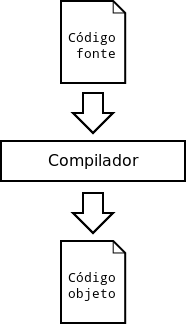
\includegraphics[width=.2\textwidth]{images/compilador.png}
%    \hspace{5em}
%    \pause
%    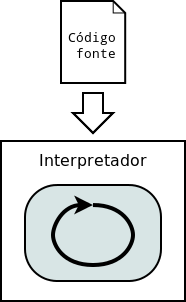
\includegraphics[width=.2\textwidth]{images/interpretador.png}
%  \end{figure}
%\end{frame}
%-------------------------------------
\section{Por trás de uma linguagem de script}
%-------------------------------------
\frame{
  \begin{center}
  \LARGE 2. Por trás de uma linguagem de \textit{script}
  \end{center}
}
%-------------------------------------
\begin{frame}[fragile]
  \frametitle{O interpretador}
  \begin{figure}
    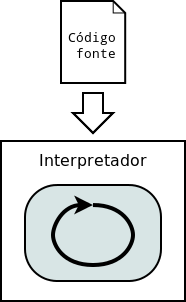
\includegraphics[height=.5\textheight]{images/interpretador.png}
  \end{figure}
\end{frame}
%-------------------------------------
\begin{frame}[fragile]
  \frametitle{Como ele funciona?}
  \begin{figure}
    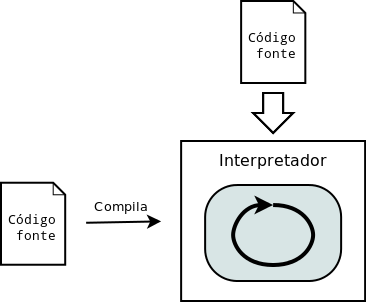
\includegraphics[height=.5\textheight]{images/nativo-vs-virtual-01.png}
  \end{figure}
\end{frame}
%-------------------------------------
\begin{frame}[fragile]
  \frametitle{Linguagem Nativa e Linguagem Virtual}
  \begin{figure}
    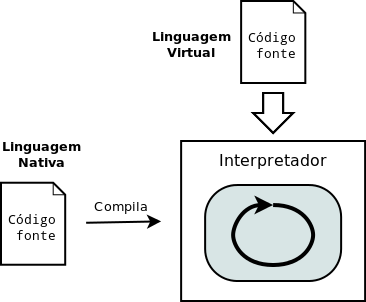
\includegraphics[height=.5\textheight]{images/nativo-vs-virtual-02.png}
  \end{figure}
\end{frame}
%-------------------------------------
\begin{frame}[fragile]
  \frametitle{A Máquina Virtual}
  \begin{figure}
    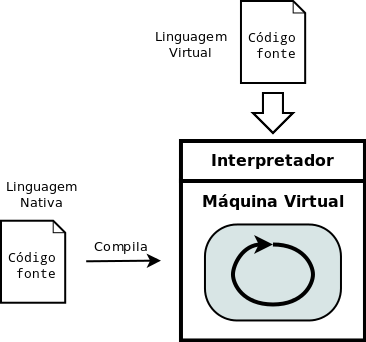
\includegraphics[height=.6\textheight]{images/nativo-vs-virtual-03.png}
  \end{figure}
\end{frame}
%-------------------------------------
\begin{frame}[fragile]
  \frametitle{A API Nativa}
  \begin{figure}
    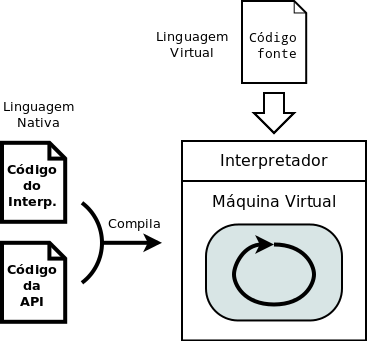
\includegraphics[height=.6\textheight]{images/nativo-vs-virtual-04.png}
  \end{figure}
\end{frame}
%-------------------------------------
\begin{frame}[fragile]
  \frametitle{Onde queremos mexer}
  \begin{figure}
    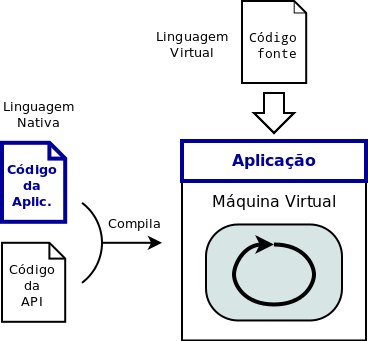
\includegraphics[height=.6\textheight]{images/nativo-vs-virtual-05.png}
  \end{figure}
\end{frame}
%-------------------------------------
\section{O Sistema}
%-------------------------------------
\frame{
  \begin{center}
  \LARGE 3. O Sistema
  \end{center}
}
%-------------------------------------
\subsection{Visão Geral}
%-------------------------------------
\frame{
  \begin{center}
  \Large 3.1. Visão Geral
  \end{center}
}
%-------------------------------------
\begin{frame}[fragile]
  \frametitle{O Problema}
  \pause
  \begin{block}{}
    Integrar, de maneira automatizada, uma linguagem nativa (\texttt{C++}) com
    mais de uma linguagem de \textit{script} (\texttt{Lua}, \texttt{Python}, ...).
  \end{block}
  \pause
  %TODO Dividir essar imagem?
  \begin{figure}
    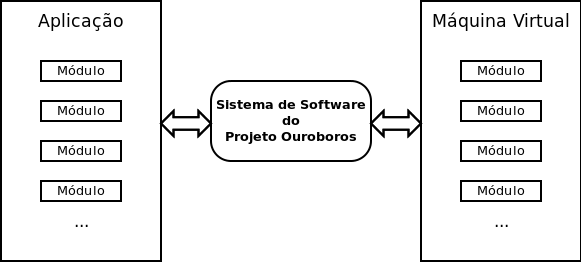
\includegraphics[width=.7\textwidth]{images/overview-simple.png}
  \end{figure}
\end{frame}
%-------------------------------------
\frame{
  \frametitle{Os casos}
  \pause
  A integração ocorre em dois sentidos:
  \begin{itemize}
    \pause
    \vspace{1em}
    \item Máquina Virtual $\Rightarrow$ Aplicação: \textbf{Incorporação}.
    \pause
    \vspace{1em}
    \item Aplicação $\Rightarrow$ Máquina Virtual: \textbf{Exportação}.
  \end{itemize}
}
%-------------------------------------
\subsection{Incorporação}
%-------------------------------------
\frame{
  \begin{center}
    \Large
    3.2. Incorporação \\
    \normalsize
    (a.k.a. \textit{embedding})
  \end{center}
}
%-------------------------------------
\begin{frame}[fragile]
  \frametitle{O que é incorporação?}
  \pause
  \begin{columns}
    \column[t]{.5\textwidth}
      \begin{block}{myscript.lua}
        \begin{lstlisting}[language=lua]
variable = 42
function foo (x, y)
  return x+y
end
        \end{lstlisting}
      \end{block}
    \pause
    \column[t]{.5\textwidth}
      \begin{block}{myscript.py}
        \begin{lstlisting}[language=python]
variable = 42
def foo(x, y):
  return x+y
        \end{lstlisting}
      \end{block}
  \end{columns}
  \pause
  \begin{block}{myprog.cxx}
    \begin{lstlisting}
ScriptManager *manager = SCRIPT_MANAGER();
// Load the script
VirtualObj myscript = manager->LoadModule("myscript");
// Gets the value 42
int script_integer = myscript["variable"].value<int>();
// Results in 9001
int result = myscript["foo"](9000, 1).value<int>();
    \end{lstlisting}
  \end{block}
\end{frame}
%-------------------------------------
\begin{frame}[fragile]
  \frametitle{Como funciona? [1] [2]}
  \pause
  \begin{block}{Incorporando com Lua}
    \begin{lstlisting}
// L is a lua_State*
lua_getfield(L, LUA_GLOBALSINDEX, "variable");
// The value is put on the top of the stack
int value = lua_tointeger(L, -1);
    \end{lstlisting}
  \end{block}
  \pause
  \begin{block}{Incorporando com Python}
    \begin{lstlisting}
// module is a PyObject*
PyObject *var = PyObject_GetAttrString(module, "variable");
// var contains the value we want
int value = PyInt_AsLong(var);
    \end{lstlisting}
  \end{block}
\end{frame}
%-------------------------------------
\frame{
  \frametitle{Interface Unificada}
  \pause
  \begin{center}
    \Large
    Ouroboros Project API \\
    (OPA)
  \end{center}
  \pause
  Principais classes:
  \begin{itemize}
    \pause
    \item \texttt{VirtualObj}: abstrai quaisquer objetos de \textit{script}.
    \pause
    \item \texttt{VirtualMachine}: abstrai cada linguagem virtual.
    \pause
    \item \texttt{ScriptManager}: gerencia as máquinas virtuais.
  \end{itemize}
  \vspace{1em}
  \pause
  \hspace{17em} Como? \pause \textbf{Polimorfismo!}
}
%%-------------------------------------
%\begin{frame}[fragile]
%  \frametitle{Implementação}
%  \pause
%  \begin{center}
%    \Large
%    Polimorfismo!
%  \end{center}
%  \pause
%  \vspace{-1em}
%  \begin{figure}
%    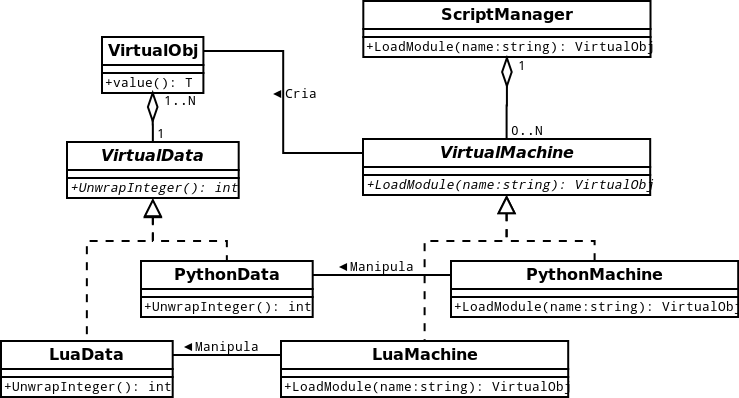
\includegraphics[width=.9\textwidth]{images/implementation.png}
%  \end{figure}
%\end{frame}
%-------------------------------------
\begin{frame}[fragile]
  \frametitle{Tipos definidos pelo Usuário}
  \pause
  E se eu quiser fazer isso?
  \pause
  \begin{block}{Usando tipo do usuário}
    \begin{lstlisting}
// Load the script
VirtualObj myscript = manager->LoadModule("myscript");
// Some object
MyClass *object = myscript["object"].value<MyClass*>();
    \end{lstlisting}
  \end{block}
  \begin{itemize}
    \pause
    \item A máquina virtual tem que conhecer \texttt{MyClass}.
    \pause
    \item Precisa lidar com herança.
    \pause
    \item Tem que gerenciar a memória.
  \end{itemize}
\end{frame}
%-------------------------------------
\subsection{Exportação}
%-------------------------------------
\frame{
  \begin{center}
    \Large
    3.3. Exportação \\
  \end{center}
}
%-------------------------------------
\begin{frame}[fragile]
  \frametitle{O que é exportação?}
  \pause
  \begin{block}{myprog.h}
    \begin{lstlisting}
class MyClass { /* ... */ };

int bar (int x) { return x+x; }
    \end{lstlisting}
  \end{block}
  \pause
  \begin{columns}
    \column[t]{.5\textwidth}
      \begin{block}{myscript.lua}
        \begin{lstlisting}[language=lua]
require 'myprog'

obj = myprog.MyClass()

print(myprog.bar(1337))
        \end{lstlisting}
      \end{block}
    \pause
    \column[t]{.5\textwidth}
      \begin{block}{myscript.py}
        \begin{lstlisting}[language=python]
from myprog import MyClass
from myprog import bar

obj = MyClass()

print(bar(1337))
        \end{lstlisting}
      \end{block}
  \end{columns}
\end{frame}
%-------------------------------------
\begin{frame}[fragile]
  \frametitle{Como funciona: Lua}
  \pause
  \begin{block}{Lua\_myprog\_wrap.cxx}
    \begin{lstlisting}
int wrap_bar (lua_State* L) {
  int arg0 = lua_tointeger(L, 1);
  lua_settop(L, 0);
  int result = bar(arg0);
  lua_pushinteger(L, result);
  return 1;
}

luaL_Reg functions[] = { { "bar", wrap_bar }, ... };

int luaopen_myprog (lua_State* L) {
  lua_newtable(L);
  luaL_register(L, nullptr, functions);
  return 1;
}
    \end{lstlisting}
  \end{block}
\end{frame}
%-------------------------------------
\begin{frame}[fragile]
  \frametitle{Como funciona: Python}
  \pause
  \begin{block}{Python\_myprog\_wrap.cxx}
    \begin{lstlisting}
PyObject* wrap_bar (PyObject* self, PyObject* args) {
  PyObject *arg0 = PyTuple_GetItem(args, 0);
  int arg0_value = PyInt_AsLong(arg0);
  int result_value = bar(arg0_value);
  PyObject *result = PyInt_FromLong(result_value);
  return result;
}

static PyMethodDef myprogmethods[] = {
  {"bar", wrap_bar, ... }, ...
};

PyMODINIT_FUNC initmyprog (void) {
  Py_InitModule("myprog", myprogmethods);
}
    \end{lstlisting}
  \end{block}
\end{frame}
%-------------------------------------
\begin{frame}[fragile]
  \begin{center}
    Como vocês podem ver... \pause É muito chato!
  \end{center}
  \pause
  \begin{center}
    \textbf{Precisamos gerar esse código automaticamente!}
  \end{center}
\end{frame}
%-------------------------------------
\frame{
  \frametitle{Primeira solução}
  \pause
  \begin{center}
    \Large
    Simple Wrapper and Interface Generator \\
    (SWIG)
  \end{center}
  \pause
  Faz o ``trabalho sujo'' para nós, mas tem problemas:
  \begin{itemize}
    \pause
    \item Não permite herança de classes exportadas.
    \pause
    \item Não reconhece certas estruturas, como classes aninhadas.
    \pause
    \item Complicações para gerenciar a memória.
    \pause
    \item Uma interface não muito agradável.
  \end{itemize}
}
%-------------------------------------
\frame{
  \frametitle{Segunda solução}
  \pause
  \begin{center}
    \Large
    Ouroboros Project Wrapper and Interface Generator \\
    (OPWIG)
  \end{center}
  \pause
  Principais partes:
  \begin{itemize}
    \pause
    \item \textit{Parser}: analisa as declarações em \texttt{C++} do usuário.
    \pause
    \item Metadados: abstraem as declarações analisadas.
    \pause
    \item Gerador: gera o código dos \textit{wrappers} com base nos metadados.
  \end{itemize}
}
%-------------------------------------
\begin{frame}[fragile]
  \frametitle{Implementação do \textit{Parser}}
  \pause
  \vspace{-1em}
  \begin{figure}
    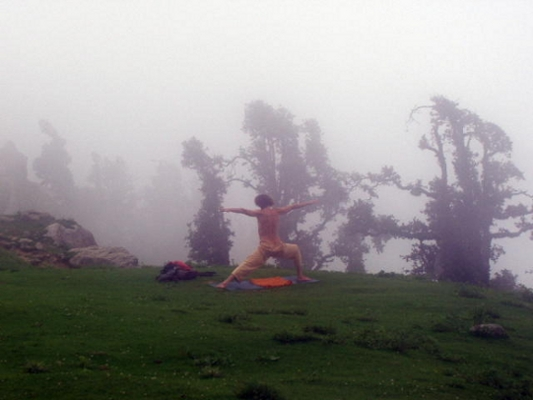
\includegraphics[width=.4\textwidth]{images/flex.jpg}
    \pause
    
\includegraphics[width=.4\textwidth]{images/bison.jpg}
  \end{figure}
  \pause
  \begin{center}
    \texttt{Flexc++} e \texttt{Bisonc++} por Frank B. Brokken [3][4]
  \end{center}
\end{frame}
%-------------------------------------
\section{Conclusões}
%-------------------------------------
\frame{
  \begin{center}
  \LARGE 4. Conclusões
  \end{center}
}
%-------------------------------------
\frame{
  \frametitle{Funciona?}
  \pause
  \begin{center}
    Testes!
  \end{center}
  \begin{itemize}
    \pause
    \item Sistema antigo: usado pelo Horus Eye e pelo Asteroids Wars.
    \pause
    \vspace{1em}
    \item \textit{Parser} e metadados: testes de unidade e de funcionalidade,
          usando \texttt{gooogletest} [5] e Travis [6].
    \pause
    \vspace{1em}
    \item OPA e OPWIG: testes de aceitação na forma de \textit{milestones}.
  \end{itemize}
}
%-------------------------------------
\frame{
  \frametitle{Dificuldades}
  \begin{itemize}
    \pause
    \item Compatibilidade com \texttt{C++11} em Windows.
    \pause
    \vspace{1em}
    \item \texttt{C++} não tem uma gramática livre de contexto.
    \pause
    \vspace{1em}
    \item Falta de planejamento no começo.
  \end{itemize}
}
%-------------------------------------
\frame{
  \frametitle{Próximos passos}
  \begin{itemize}
    \pause
    \item Lançamento oficial (organizar repositórios, criar página oficial...)
    \pause
    \vspace{1em}
    \item Incrementar o \textit{parser} e o gerador para ele reconhecer
          \texttt{C++} completamente (incluindo \texttt{C++11})
    \pause
    \vspace{1em}
    \item Dar suporte a mais linguagens!
    \pause
    \vspace{1em}
    \item Explorar usos alternativos com programação reflexiva em \texttt{C++}
  \end{itemize}
}
%-------------------------------------
\section{Unlimited slide works}
%-------------------------------------
\begin{frame}
  \begin{center}
    \LARGE Obrigado!
  \end{center}
\end{frame}
%-------------------------------------
\begin{frame}
  \frametitle{Bibliografia}
  \begin{itemize}
    \footnotesize
    \item[1]
      Lua C API. http://www.lua.org/manual/5.1/manual.html\#5, Novembro 2013.
    \vspace{1em}
    \item[2]
      Python C API. http://docs.python.org/2/c-api/, Novembro 2013.
    \vspace{1em}
    \item[3]
      Frank B. Brokken. http://flexcpp.sourceforge.net/, Novembro 2013.
    \vspace{1em}
    \item[4]
      Frank B. Brokken. http://bisoncpp.sourceforge.net/, Novembro 2013.
    \vspace{1em}
    \item[5]
      Google. https://code.google.com/p/googletest/, Novembro 2013.
    \vspace{1em}
    \item[6]
      Travis CI. https://travis-ci.org/, Novembro 2013.
  \end{itemize}
\end{frame}
%-------------------------------------
\end{document}

